\chapter{课题介绍}

\section{EAST}
EAST (\textbf{E}xperimental \textbf{A}dvanced \textbf{S}uperconducting \textbf{T}okamak) 实验先进超导托卡马克位于合肥等离子体物理研究所。

\begin{table}[htb]
    \centering
    \caption{\east 设计参数}
    \label{tab:east_parameter}
    \begin{tabularx}{\linewidth}{lXlXlX}
        \toprule[1.5pt]
        $R$ 大半径 &   & $a$ 小半径 &  & $\delta$ 三角形变系数 & \\
        $B_t$ 环向中心磁感应强度 &   & *** &  & *** & \\
        % \midrule[1pt]
        \bottomrule[1.5pt]
    \end{tabularx}
\end{table}

\section{边界局域模}
边界局域模 (Edge Localize Mode, ELM) 是一种在\Hmode 等离子体中存在的磁流体不稳定性,相比于\Lmode 等离子体,\Hmode 等离子体边界密度梯度和温度梯度更为显著,当梯度达到阈值时,等离子体边界会间歇性地将能量和粒子从边界脉冲式地释放出去,周而复始。\Hmode 最早在ASDEX 托卡马克上被发现了,其特点在于边界压强梯度较大,从而形成台基区(pedestal)。ELM 在 \ddd 上得到了充分的研究,其分类很大程度上受到了 \ddd 的影响,其提出的 。不过 ELM 并不是完全不好,重复可控的边界局域模发生也可以帮助控制等离子体中的粒子存量。



边界局域模相关的理论难以给出能量和粒子损失速率的定量描述,于是便很难和实验的对比。可以比较的是实验观测到的时间尺度,例如,边界局域模的上升时间尺度,持续时间尺度以及在以及边界局域模重复频率的变化趋势,另外,边界局域模发生的径向范围可以用理论给出,而且可以和实验的发现进行一个对比。

从目前聚变等离子体中 ELM 现象来看,\cite{zohm_edge_1996} 将其清晰地划分为三种。


\begin{itemize}
    \item \textit{\typeone ELM}  重复频率 $\nu_{ELM}$ 随着加热功率的增加而增加。在高温时,\typethr 的 ELM 已经被抑制住了,此时理想气球模限制了可以达到的边界最大压力梯度 $\alpha/\alpha_{\text{crit}}\approx 1$,如果理想气球模耦合了一种低 $n$ 的不稳定性(由于强边界电流密度,很有可能是一种类扭结的不稳定性),\typethr ELM 就会发展起来。如果通过等离子体塑形可以使等离子体边界符合气球模的第二类稳定域,那么该类型 ELM 就会被抑制住,而此时对边界压力梯度的限制,就将由低 $n$ 的磁流体不稳定性所决定。\\
    ELM 在目前的实践中,没有显著的磁前兆振荡被检测到,不过这类 ELM 发生之前会有密度湍流波动的增强。这类不稳定性会使得 $D_\alpha$ 信号产生间断的剧烈爆发。
    \item \textit{\typethr ELM} 重复频率 $\nu_{ELM}$ 随着加热功率的增加而减小.在 L-H 转换之后,在边界的电子温度不太高的情况下,由于边界输运壁垒的存在,边界的压力梯度和电流密度变得更加强烈,构成了有阻磁流体不稳定性的自由能的源头。但随着输入功率增高,足够高的温度使阻尼效应可忽略时,\typethr ELM 会被抑制住。\\
    可以通过赤道面的磁探针获得其前兆磁湍动,频率范围 $\nu_{\text{prec}}\approx \SI{50}{\kilo\hertz} \sim \SI{70}{\kilo\hertz}$ 。等离子体边界压力梯度显著低于理想气球模的极限,即 $0.3\leq \alpha/\alpha_{\text{crit}}\leq 0.5$。
    \item \textit{Dithering Cycles, 振荡循环型} 在 L-H 转换过程中,由于\Hmode 功率的滞后而在阈值上下而往复的循环是有可能的。边界的压力和电流梯度和 \Lmode 时类似,所以可以说,振荡周期型不是一种典型的磁流体不稳定性,而是一种 L-H-L 模转换连续发生的现象。
\end{itemize}

尽管受 ELM 复杂的非线性物理所限,这样的物理描述不能作为一种 ELM 的精确定义。但这种唯象的理解是基于实验观测到的结果,并且和目前对磁流体稳定性的分析相差不甚。



\cite{2003PPCF...45.1549L} 基于目前装置上实验参数的外推结果,\iter 上 \typeone ELM 可能会导致损失 $5\sim \SI{22}{\mega\joule}$ ,其中约一半分布在 $\sim \SI{1}{\meter^2}$ 壁上的热沉积范围\inlinecite{Loarte_2014}。壁材料瞬态接受的能量密度在 $2.5\sim \SI{11}{\mega\joule/\meter^2}$,是目前材料(钨或碳纤维材料)承受热负荷能力的 $5\sim 20$ 倍。如何控制或者抑制 ELMs 成为了相当关键的一个问题。由共振磁扰动(RMP)引起的共振及边界随机场被认为可以抑制在等离子体边界周期性或拟周期性的破裂。


不过等离子体对扰动的响应往往会屏蔽掉 RMP 线圈施加的影响并且大大地降低磁场的随机程度\inlinecite{sun_nonlinear_2016},这使得通过 RMP 线圈有效可靠地抑制边界局域模 ELM 需要深入的研究。

目前学界对 ELM 的弱化和抑制之间的关键区别还不明晰,同时等离子体对 ELM 抑制的线性/非线性响应均有待探索。

\section{本课题中涉及的扰动场}

在聚变等离子体中用到的外加扰动场(magnetic perturbation, MP)是指螺旋形或鞍形线圈产生的量级为 $\delta B_r/\delta B_t=10^{-5}\sim 10^{-3}$ 的磁场扰动。将外加磁扰动在磁面坐标系中并进行空间傅里叶分解运算,可以得到多个极向模数为 $m$, 环向模数为 $n$ 的分量。其分布在 $q_{min}<m/n<q_a$ 分量螺旋程度与安全因子为 $q_s=m/n$ 的有理面相同的螺旋度,从而可以实现通过共振效应对有理面上的不稳定性造成较大影响。因此,磁扰动中的这些分量特别地命名为共振磁扰动(Resonant Magnetic Perturbation, RMP)。RMP 使得其在某个特定的磁面产生共振(通常指等离子体边界区域)。这里共振指的是在目标磁面施加的径向磁场螺旋度和平衡场的相近。

RMP 的目的在于稳定 ELM,避免脉冲式的粒子流和热负荷,使得直面等离子体的材料能够长时间工作。


\subsection{腔内低场侧 RMP}
一套 RMP 线圈系统于 2014 年安装在 EAST 的低场侧,它包含有两组线圈($2*8=16$)。EAST 团队通过扰动场环向模数为 $n=1, 2$ 的 RMPs 实现了 \typeone 边界局域模的弱化和完全的抑制。

\subsection{高 m 线圈}
等离子体所新近研发的高 m 线圈 \inlinecite{zhang_highm} 激发出的扰动场有着高 m,宽 n 特征,分为上下对称两组($2*2=4$),几何最大电流为 \SI{5}{\kilo\ampere}。 
物理计算过程中采用的线圈几何尺寸如图 \ref{fig:highm-pos} 所示。其对等离子体的影响现正被研究,由于高 $m$ 线圈组设计位于一个极向截面内,即 $\phi\equiv \text{const}$ 处,其对等离子体的影响局域性很明显,此类强局域性扰动磁场对等离子体边界稳定性的影响也可以从中得到研究。

采用与现有 RMP 系统相同线圈材料 线圈位置位于低场侧限制器后方,利用限制器作为线圈的保护,尽可能靠近等离子体 


\begin{figure}[htbp]
    \centering%
    % \hspace{4em}%
    \begin{subfigure}{0.45\textwidth}
      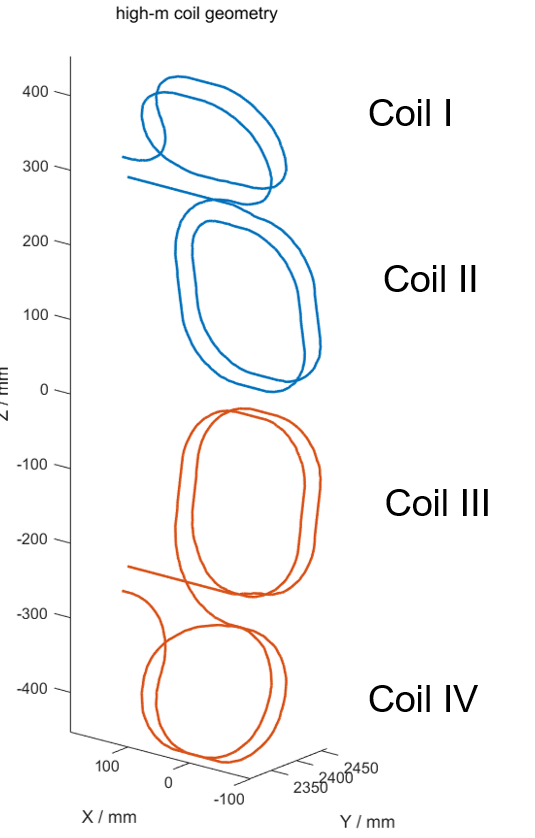
\includegraphics[height=8cm]{highm/coil_geometry.png}
      \caption{高 $m$ 线圈的立体几何位置}
    \end{subfigure}
    % \hspace{4em}%
    \begin{subfigure}{0.45\textwidth}
      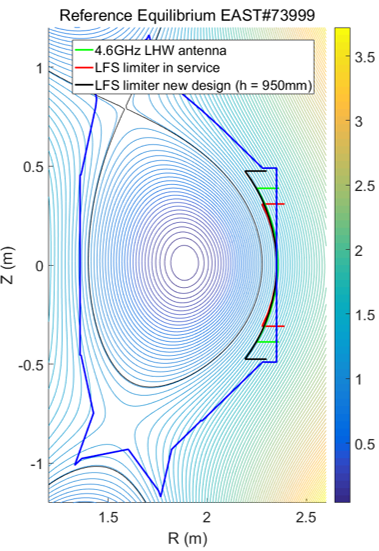
\includegraphics[height=8cm]{highm/coil_limiter_pos.png}
      \caption{极向截面上高 $m$ 线圈的位置}
    \end{subfigure}
    \caption{高 $m$ 线圈在 \east 中的设计和所处的几何位置,来源于张华祥研究员 \cite{zhang_highm} 的报告}
    \label{fig:highm-pos}
  \end{figure}

根据两组线圈内电流的相对方向,有两种工作模式,见图 \ref{fig:highm-pos}。\textit{主要工作模式}时两组线圈通同向电流;\textit{次要工作模式}时则反向。



\begin{figure}[htbp]
    \centering%
    \begin{subfigure}{0.33\textwidth}
      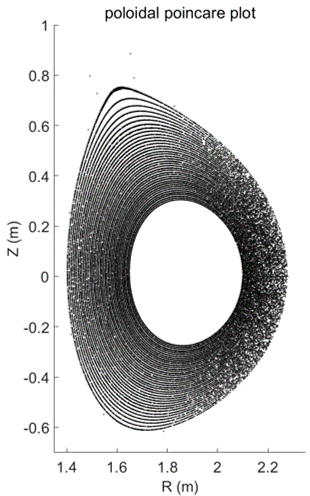
\includegraphics[height=8cm]{highm/original_equilibrium_no_high_m.png}
      \caption{平衡场}
    \end{subfigure}%
    % \hspace{4em}%
    \begin{subfigure}{0.33\textwidth}
      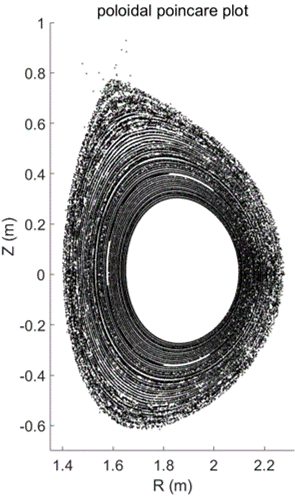
\includegraphics[height=8cm]{highm/original_equilibrium_with_high_m.png}
      \caption{主要工作模式的线圈场}
    \end{subfigure}
    % \hspace{4em}%
    \begin{subfigure}{0.33\textwidth}
      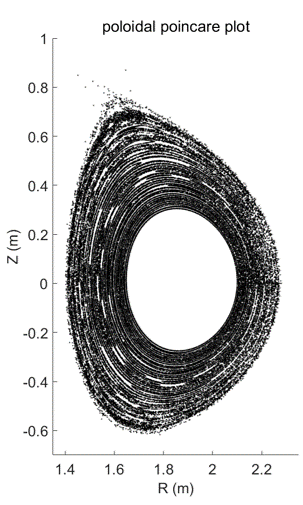
\includegraphics[height=8cm]{highm/original_equilibrium_with_high_m_inverse.png}
      \caption{次要工作模式的线圈场}
    \end{subfigure}
    \caption{高 m 线圈作用下的平衡场扰动情况,次要工作模式下的磁扰动情况较主要模式更深,来源于张华祥研究员 \cite{zhang_highm} 的报告}
    \label{fig:highm-three-subfig-poincare}
  \end{figure}

  
\begin{figure}[htbp]
    \centering%
    % \hspace{4em}%
    \begin{subfigure}{0.8\textwidth}
        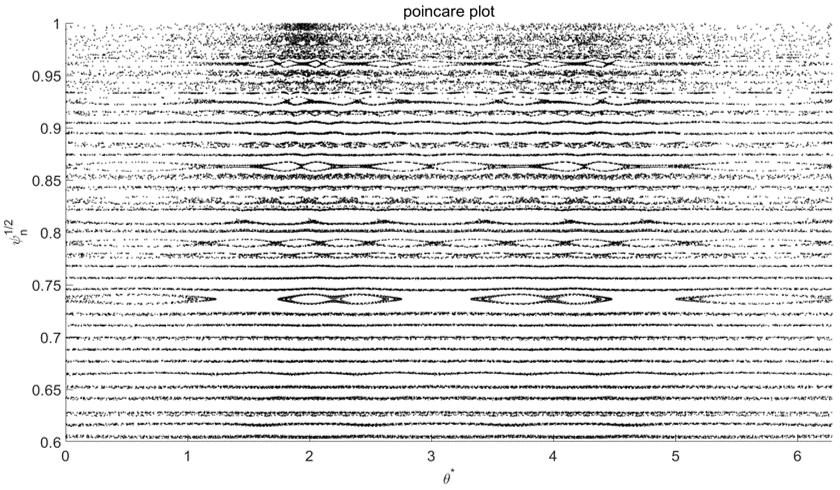
\includegraphics[height=6.6cm]{highm/stretched_poincare_primary_state.png}
        \caption{高 $m$ 线圈主要工作模式下展开的 \Poincare 图}
    \end{subfigure}
    % \hspace{4em}%
    \begin{subfigure}{0.8\textwidth}
        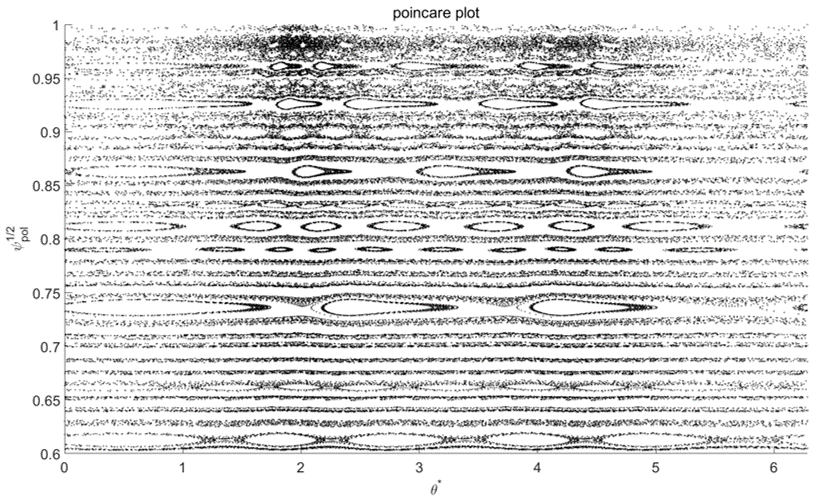
\includegraphics[height=6.6cm]{highm/stretched_poincare_secondary_state.png}
        \caption{高 $m$ 线圈次要工作模式下展开的 \Poincare 图}
    \end{subfigure}
    \caption{高 $m$ 线圈作用下的 \Poincare 图,次要工作模式下的磁扰动情况较主要模式更深,来源于张华祥研究员 \cite{zhang_highm} 的报告}
    \label{fig:highm-stretched-poincare}
\end{figure}
  

% \begin{figure}[H] % use float package if you want it here
%     \centering
%     \includegraphics{thu-whole-logo.pdf}
%     \caption{利用 Xfig 制图}
%     \label{fig:xfig1}
% \end{figure}







\subsection{低杂波驱动的螺旋电流丝}
RMP 其致命的弱点是线圈置于腔内,这在 DEMO 堆的设计中是不被允许的,研究人员只能通过其他手段来改变边界磁拓扑。 在低杂波加热设计之外得到的螺旋电流丝,是一个很有吸引力的在下一代聚变设备中应用的 RMP 手段。

低杂波加热原本用于芯部等离子体电流驱动,它通过朗道阻尼将动量传给等离子体,可以实现不依赖于离子回旋共振加热 (ICRH) 的长脉冲\Hmode 运行。但在原本被设计好的加热作用之外,还在 \ddd、\east 等不同装置上发现了低杂波驱动的螺旋电流丝,低杂波启动后毫秒内电流丝即响应出现,电流丝数量和托卡马克中低杂波天线的行数相同。


\begin{figure}[htbp]
    \centering%
    % \hspace{4em}%
    \begin{subfigure}{0.45\textwidth}
        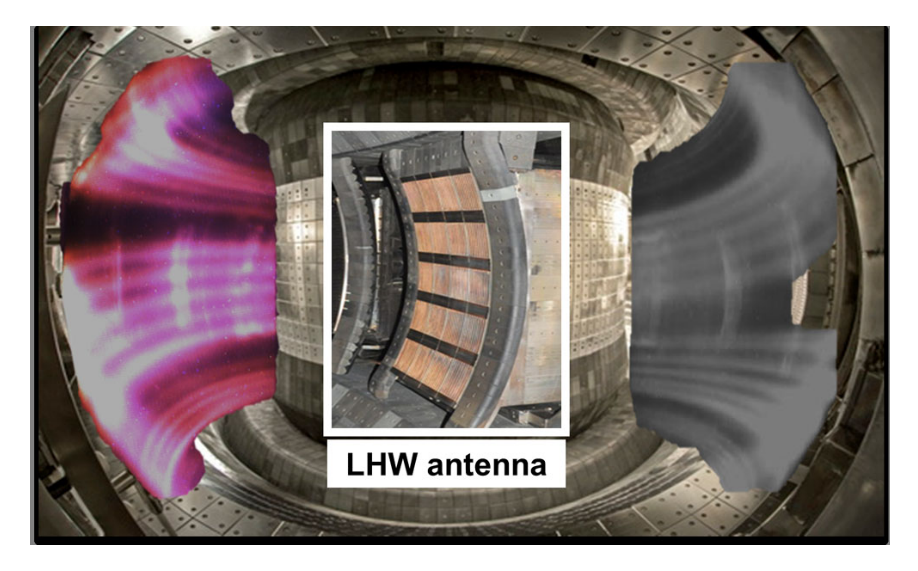
\includegraphics{hcf/hcf_visible_image.png}
        \caption{\east 以氦气放电实验来用可见光显著地表现螺旋电流丝的三维几何分布,低杂波天线截图置于图中间。}
    \end{subfigure}
    % \hspace{4em}%
    \begin{subfigure}{0.45\textwidth}
        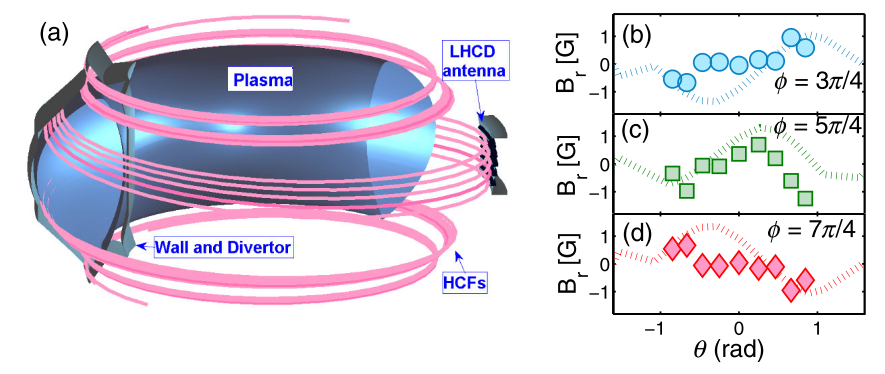
\includegraphics{hcf/hcf_model_sketch.png}
        \caption{对低杂波激发的螺旋电流丝以图 (a) 中的电流分布进行了模拟,计算结果得到环向非对称的磁扰动径向分布,图中显示了 (b) $\phi=3\pi/4$  (c) $\phi=5\pi/4$  (d) $\phi=7\pi/4$ 的计算和实验结果。极向角 $\phi$ 在低场侧赤道面为零顺时针方向增长;从上往下看托卡马克,环向角 $\phi$ 在低杂波天线处为零逆时针方向增长。}
    \end{subfigure}
    \caption{高 $m$ 线圈作用下的 \Poincare 图,次要工作模式下的磁扰动情况较主要模式更深,来源于张华祥研究员 \cite{zhang_highm} 的报告}
    \label{fig:highm-stretched-poincare}
\end{figure}
  

在 EAST 中为了研究低杂波及螺旋电流丝,以方波调制的低杂波功率进行了间断性的螺旋电流丝激励 \inlinecite{the_east_team_magnetic_2013}。低杂波天线运转时,螺旋电流丝引起的三维磁拓扑(磁连接长度计算如图 \ref{fig:hcf-connection}) 导致了粒子流三维分裂的落点图案。\cite{the_east_team_magnetic_2013}

\begin{figure}[htbp]
    \centering%
        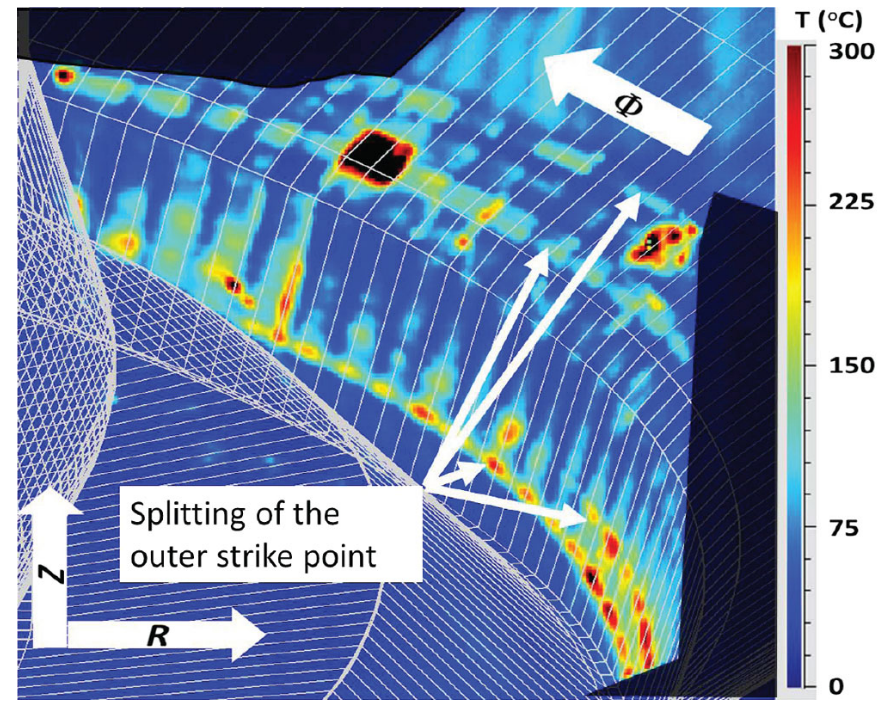
\includegraphics[height=9cm]{hcf/splitting_strike_point_ir.png}
        \caption{红外摄像机分析得到的\east 外侧偏滤器平板上$\phi=1.3\pi\sim 1.5\pi$低杂波运转时的温度分布。图中可见落点分裂为多个条状加热图案,还可以发现环向上分布的不对称性。腔壁网格重叠在图中以白线显示环形腔结构。}
        \label{fig:hcf-strike-point}
\end{figure}

\begin{figure}[htbp]
    \centering%
        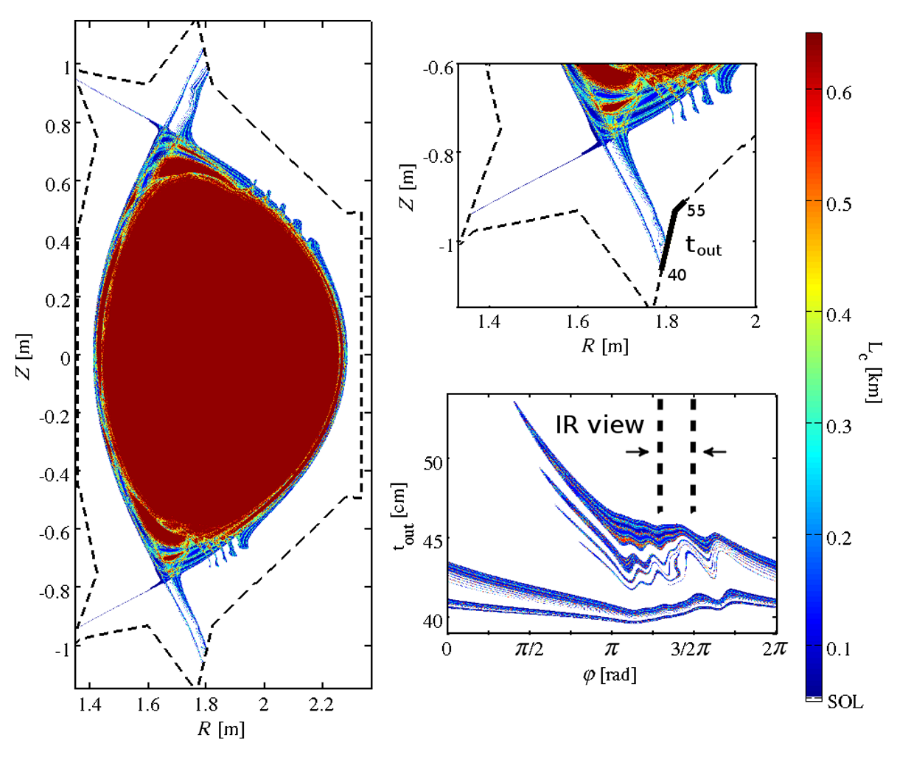
\includegraphics[height=9cm]{hcf/connection_contour.png}
        \caption{用上图 \ref{fig:hcf-strike-point} 实验中测量值重建的 \east 中磁连接长度在极向截面 $\phi=1.3\pi$ 上的等位线分布,其下偏滤器处的分布可见用右上小图。对落点的分布计算可见右下小图,右图 \ref{fig:hcf-strike-point} 红外拍照区域在小图中标注。}
        \label{fig:hcf-connection}
\end{figure}


\section{\Poincare 图及傅里叶模数分析}
\Poincare 图是对磁面结构的描述,通过在给定极向截面上进行沿磁力线的迭代来标记在同一磁面上的点,以描绘出磁面的嵌套结构。

\section{数值计算工具}
\subsection{有限元、有限体积法}
偏微分方程的求解问题构成了现代工程领域许多重要的设计工作,计算框架和数值理论在各种高性能计算处理器的基础上的组合计算成为了现代工业设计的重要设计及优化工作。

有限元法(Finite Element Method, FEM)在多物理场分析中很成功,一方面它非常通用,另一方面有限元可以对不同计算域内物理问题适合的算法进行组合,这对于多物理问题而言是一个关键优势。

尽管有限元可以自然地处理弯曲和不规则几何图形,但有限元背后的数学相对有限体积法(Finite Volume Method, FVM)更复杂一些。有限体积法中自然地对物理偏微分方程组中的守恒量进行在网格上进行积分,离散值表示的是单元内该守恒量的积分平均值。于是有限体积法的重点在于如何通过单元(cell)的积分平均值插值表示单元边界的守恒量流量,即流函数。

% 最后,对于时域时间上的仿真,为了效率往往需要使用显式求解器。但是有限元在实施此类技术方面存在困难,因此建议不要使用它。

\begin{itemize}
    \item 等离子体所采用的电磁场计算软件 TODO
    \item \textit{FEniCS\footnote{\url{https://fenicsproject.org/}}} 是开源(LGPLv3)的偏微分方程计算框架。 FEniCS 中丰富的 Python-C++ 接口使得科学工作者可以迅速地将他们面对的科学模型转化为有限元程序逻辑。在这里我们选取 FEniCS 是因为其后端的 PETSc\footnote{\url{https://www.mcs.anl.gov/petsc/}} 在支持 OpenMP、OpenCL 和 CUDA,在针对 PDE 的硬件优化上几乎无出其右,可以在几乎在任何并行计算硬件平台上得到快速应用。\underline{考虑到毕设时间的有限并且可能将考虑非线性等离子体响应},具备高层接口的 FEniCS 是快速实现偏微分方程的手段\inlinecite{FEniCS_LangtangenLogg2017}。
    \item \textit{SU2\footnote{\url{https://su2code.github.io}}} 工具箱是基于 C++ 偏微分方程的求解分析工具并可以在给定条件基础上进行设计优化。这套工具是为计算流体力学和空气动力学形状优化而设计的,但它也能够进行扩展来处理任意几何的控制方程,例如位势流,弹性问题,电流力学问题,化学反应流以及其他问题。
    \item \textit{MFEM\footnote{\url{https://mfem.org/}}} 与 FEniCS 类似,MFEM 也支持对后端采用 PETSc 进行并行加速。其在电磁场领域有过一些研究,在本论文中被采用作为辅助验证工具。
    \item \textit{\mdddc \footnote{\url{https://w3.pppl.gov/~nferraro/m3dc1.html}}} 由美国普林斯顿大学等离子体实验室开发,是一个聚变等离子体界影响深远的非线性双流体模拟计算工具。但由于中美关系恶化及其代码闭源问题,\mdddc 的数值高精度算法及各类成果在本论文中仅作为数值理论的参考。
\end{itemize}



以下为 \mdddc 中的双流体模型方程,其推导过程参见附录。TODO
\begin{equation}\begin{aligned}
    \frac{\partial n}{\partial t}+\nabla \cdot(n \vect{u})=& 0 \\
    n m_{i}\left(\frac{\partial \vect{u}}{\partial t}+\vect{u} \cdot \nabla \vect{u}\right)=& \vect{J} \times \vect{B}-\nabla p-\nabla \cdot\tens{\Pi}+\vect{F} \\
    \frac{\partial p}{\partial t}+\vect{u} \cdot \nabla p+\Gamma p \nabla \cdot \vect{u}=&(\Gamma-1)\left[Q-\nabla \cdot \vect{q}+\eta J^{2}-\vect{u} \cdot \vect{F}-\tens{\Pi}: \nabla u\right] \\
    &+\frac{1}{n e} \vect{J} \cdot\left(\frac{\nabla n}{n} p_{e}-\nabla p_{e}\right)+(\Gamma-1) \tens{\Pi}_{e}: \nabla\left(\frac{1}{n e} \vect{J}\right) \\
    \frac{\partial p_{e}}{\partial t}+\vect{u} \cdot \nabla p_{e}+\Gamma p_{e} \nabla \cdot \vect{u}=&(\Gamma-1)\left[Q_{e}-\vect{q}_{e}+\eta J^{2}-\vect{u} \cdot \vect{F}_{e}-\tens{\Pi}_{e}: \nabla u\right] \\
    &+\frac{1}{n e} \vect{J} \cdot\left(\frac{\nabla n}{n} p_{e}-\nabla p_{e}\right)+(\Gamma-1)\left[\tens{\Pi}_{e}: \nabla\left(\frac{1}{n e} \vect{J}\right)+\frac{1}{n e} \vect{J} \cdot \vect{F}_{e}\right]
\end{aligned}\end{equation}

\begin{table}[htb]
    \centering
    % \caption[模板文件]{模板文件。如果表格的标题很长,那么在表格索引中就会很不美
    %   观,所以要像 chapter 那样在前面用中括号写一个简短的标题。这个标题会出现在索
    %   引中。}
    \label{tab:formula_double-fluid}
    \begin{tabularx}{\linewidth}{lXlXlX}
        % \toprule[1.5pt]
        $p,p_e$ &  总/电子压强 & $\vect{q}$ & 热流密度 & $\vect{J}$ & 电流密度\\
        $\tens{\Pi},\tens{\Pi}_e$ & 总/电子粘性系数 &$u$ & 流体速度 & $n$ & 粒子数密度 \\
        $\vect{F},\vect{F}_e$ & &$\tens{\Pi}$ & & $Q,Q_e$ & 
        % \midrule[1pt]
        % \bottomrule[1.5pt]
    \end{tabularx}
\end{table}

\begin{equation}
\vect{E}=\eta \vect{J}-\vect{u} \times \vect{B}+\frac{1}{n e}\left(\vect{J} \times \vect{B}-\nabla p_{e}-\nabla \cdot \tens{\Pi}_{e}+\vect{F}_{e}\right)\end{equation}

\begin{equation}\begin{aligned}
    \vect{J} &=\frac{1}{\mu_{0}} \nabla \times \vect{B} \\
    \frac{\partial \vect{B}}{\partial t} &=-\nabla \times \vect{E}
\end{aligned}\end{equation}

\mdddc 中还有单流体模型, \cite{canal_m3d-c1_2017} 对 NSTX-U 中等离子体对扰动场的响应做了稳态单/双流体模拟的对比。

\begin{equation}\begin{aligned}
    \nabla \cdot\left(n \vect{v}_{\mathrm{i}}\right)=&0\\
    m_{\mathrm{i}} n \vect{v}_{\mathrm{i}} \cdot \nabla \vect{v}_{\mathrm{i}}=&\vect{J} \times \vect{B}-\nabla p-\nabla \cdot \tens{\Pi}_{\mathrm{i}}\\
    \frac{\nabla \cdot\left(p \vect{v}_{\mathrm{i}}\right)}{\Gamma-1}+p \nabla \cdot \vect{v}_{\mathrm{i}}+\nabla \cdot \vect{q}=&\eta J^{2}-\tens{\Pi}_{\mathrm{i}}: \nabla \vect{v}_{\mathrm{i}}-\frac{\vect{J}}{n e(\Gamma-1)} \cdot\left(\Gamma p_{\mathrm{e}} \frac{\nabla n}{n}-\nabla p_{\mathrm{e}}\right)\\
    \nabla \times \vect{E}=&0\\
    \nabla \times \vect{B}=&\mu_{0} \vect{J}
\end{aligned}\end{equation}

\begin{equation}\vect{E}=\eta \vect{J}-\vect{v}_{\mathrm{i}} \times \vect{B}+\frac{1}{n e}\left(\vect{J} \times \vect{B}-\nabla p_{\mathrm{e}}\right)\end{equation}

\begin{equation}\tens{\Pi}_{i}=-\mu_{i}\left[\nabla \vect{v}_{i}+\left(\nabla \vect{v}_{i}\right)^{t}\right]\end{equation}

\begin{equation}\vect{q}=-\kappa \nabla\left(T_{e}+T_{\mathrm{i}}\right)-\kappa_{\|} \vect{B}\left(\vect{B} \cdot \nabla T_{\mathrm{e}}\right) / B^{2}\end{equation}

\subsection{质点网格法 Particel-in-cell (PIC)}

在以上的偏微分方程求解时,物理问题允许将某一点(或一个邻域内)的物理量取其代表值来离散化,如有限体积法中取其网格内的平均值进行计算,,有限元法中取有限阶多项式逼近。然而,在并不一定完全服从高斯速度分布的等离子体物理研究中,这样的代表值很难抽取出来。类似的非高斯型速度分布导致的流体假设不成立的问题,在裂变堆中子物理计算中采用的是多群计算的方法;而在聚变等离子体物理问题中,不论是自然产生的等离子体还是人工产生的加速器,往往会出现相当各向异性的速度分布,以至于需要细致地考虑在相空间中求解。对粒子在相空间(Phase space)中的分布函数 $f(\vec{x},\vec{v},t)$,描述其演化规律的物理方程是 Boltzmann 方程,\cite{ColonnaBoltamann10.1088/978-0-7503-1200-4ch1}.

\begin{equation}
\label{eq:Boltzmann}
\frac{\partial f_{s}(\vec{r}, \vec{v}, t)}{\partial t}+\left[\vec{v} \cdot \nabla_{r}+\vec{a}(\vec{r}) \cdot \nabla_{v}\right] f_{s}(\vec{r}, \vec{v}, t)=\left(\frac{\delta f_{s}}{\delta t}\right)_{\mathrm{coll}}
\end{equation}

其中 $(\delta f_{s}/\delta t )_{\mathrm{coll}}$ 表示同种粒子及不同粒子之间的相互碰撞导致的粒子 s 的 $f_s$ 变化率。
Particle-in-cell, 即 PIC 手段将电磁场进行常规的偏微分方程求解,另外,还令网格中分布着巨粒子。巨粒子对网格角点处的电磁场参数数值有所影响,同时巨粒子也会根据离散的电磁场计算其下一时间步长的速度和坐标,这样就一定程度上在完全的粒子模拟和有限网格计算方法之间达到所需要的性能、准确之间的平衡。

\subsection{磁力线定迹}
针对聚变磁约束中的磁力线定迹问题 (field-line-tracing) 和射线定迹问题 (ray-line-tracing) ,相空间中的复杂计算可以在 PIC 基础上根据磁约束的特点进行简化。以下介绍 CompX \footnote{
Computational Modeling and Software Development\url{http://compxco.com/index.html}}项目中的代码 GENRAY 和 CQL3D\footnote{它们实在太古老了,如果可以的还是把它们用 C++ 重写一遍吧}。项目中用它们作为磁力线定迹的工具。

\subsubsection{GENRAY}
GENRAY 通过几何光学式的折射处理对射线进行迹线追踪和强度变化的检索。


\subsubsection{CQL3D (Collisional QuasiLinear 3 D)}

\begin{multline}
\frac{d f}{d t}=\text{total derivative following the particle guiding center,}
=\frac{\partial f}{\partial t}+\underline{v}_{\mathrm{g.c.}} \cdot \frac{\partial f}{\partial \underline{r}}+\frac{\partial f}{\partial \mu} \frac{d \mu}{d t}+\frac{\partial f}{\partial \varepsilon} \frac{d \varepsilon}{d t}
\end{multline}


\begin{equation}\frac{d f}{d t}=\frac{\partial f}{\partial t}+v_{\|} \hat{b} \cdot \nabla f+q E_{\|} v_{\|} \frac{\partial f}{\partial \varepsilon}+O(\delta)\end{equation}

\section{磁流体不稳定性}
磁流体不稳定性高度依赖于其边界磁面的螺旋形态,而为了阐述磁面的螺旋度,旋转变换的相关知识是必需的。\textbf{旋转变换}(rotational transform, 本质上是磁面磁力线螺距角)的定义是磁力线绕环向方向转一圈时极向绕小半径转的圈数。假如磁面是互相嵌套的话,旋转变换率在磁面上的平均值由极向磁通随环向磁通的变化率决定。
$ \iota/2 \pi = d\Psi /d \Phi $。

但托卡马克中,其倒数 \textbf{安全因子} 却更常被使用,$q = 2\pi/\iota$。在截面圆形,主要由等离子体电流产生极向场的托卡马克中磁力线的方程近似满足 $ \frac{r d\theta}{B_\theta} = \frac{Rd\phi}{B_\phi} $,
其中 $ \phi $ and $\theta$ 分别是环向角和极向角。 于是在典型的托卡马克中, $ q = m/n = \left \langle d\phi /d\theta \right \rangle $ 可以用 $ q \simeq \frac{r B_\varphi}{R B_\theta} $ 近似。如果磁面安全因子 $q\leq 2$,边界上会发生显著的磁流体不稳定性。

在带偏滤器的托卡马克中,$q$ 在等离子体分界面某些部分趋近无穷,所以通常会考虑在分界面内侧的 $q$,通常来说会选 95\% 的磁面 (内部磁通占总环向磁通的 95\%), 此时常用 $q_{95}$ 来表示.




​\section{主要目标}
为了探究解决目前的\Hmode 等离子体所面临的 ELM 脉冲式热流和粒子流问题,而这在 DEMO 堆中是不被允许的。

为更好地控制 ELM, EAST 上先后测试了共振磁扰动线圈 RMP、高 m 线圈和低杂波驱动的螺旋电流丝,这三种扰动场产生机制有所差异,适用的范围也不尽相同。为了使扰动场相互配合达到最优的弱化乃至抑制边界局域模的效果,对它们在等离子体边界造成的扰动场协同作用的研究是很有必要的。 \textit{\textbf{(1)}} \textbf{腔内低场侧低 $n$ 线圈},该线圈布置在腔内,由它激发起环向模数为 $n=1,2$ 的扰动场后在 \east, \ddd 等托卡马克装置上验证了其抑制边界局域模的效应。 \textit{\textbf{(2)}} \textbf{高 m 线圈},是 EAST 团队近两年实验中的线圈,在等离子体环外加上一组四个的线圈,它的特征是扰动场环向模数 n 分布较宽,极向模数 m 较高,由于只分布在一个环向位置 $\varphi=\text{const}$,扰动场的局域性很强。 \textit{\textbf{(3)}} 由低杂波驱动的\textbf{螺旋电流丝},低杂波原本用于以朗道阻尼驱动芯部等离子体的电流,但在设计之外,实验发现它在等离子体边界会激发出螺旋电流丝,电流丝产生具体的物理机制还不甚明晰,但其亦具备调节边界磁拓扑的能力。由于低杂波天线不像共振磁扰动线圈在腔内,它具有应用在 DEMO 堆及日后商业堆的潜力。

本文将会对边界磁拓扑在扰动场作用下的变化做出(磁流体)电磁分析,绘制近边界磁面的傅里叶谱和 \Poincare 图,这构成了第二章的主要内容。在此之后,第三章将基于磁场弥散来进行粒子扩散的模拟,对粒子在边界上的运动建立直观的认识,通过修改 GENRAY-CQL3D 磁力线定迹程序可以较原来的模型更为精确。通过前面提到的多种扰动场对等离子体边界拓扑进行调节,从而对热负荷和粒子流在偏滤器上的分布进行优化,以避免脉冲式的 ELM 崩溃对壁材料造成显著的影响。最后,(如果还有时间的话Optional),通过在模拟工具中引入等离子体反馈后的随机场的计算,从而在湍流输运的角度解释磁场边界拓扑对粒子输运和热流的影响。

本论文着重在通过模拟的手段对现有的多种三维磁场进行模拟仿真,他们的磁谱被设计用来弱化或者调节边界局域模的发生。但他们之间的同时作用可以如何达到对粒子束流和热流的调节作用。